% Right dihedral alpha-PQ-beta; A on PQ; B in alpha; C in beta.
% Triangle CAB with BC perpendicular to PQ (to be proved, drawn as in original).
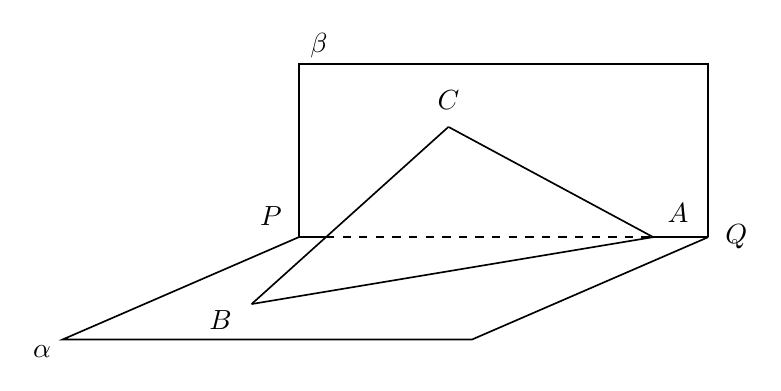
\begin{tikzpicture}[x=1cm,y=1cm,font=\normalsize,
  solidedge/.style={solid,line width=.6pt},
  hidedge/.style={dashed,line width=.6pt},
  ptlabel/.style={font=\normalsize,inner sep=2pt}]
% vertical plane beta (rectangle)
\coordinate (P) at (0,1);
\coordinate (A) at (4.5000000000,1.0000000000);
\coordinate (Q) at (5.2000000000,1.0000000000);
\coordinate (betaTL) at (0,3.2);
\coordinate (betaTR) at (5.2,3.2);
\coordinate (C) at (1.9,2.4);
% horizontal plane alpha (parallelogram)
\coordinate (alpL) at (-3.0,-0.3);
\coordinate (alpM) at (2.2000000000,-0.3000000000);
\coordinate (B) at (-0.6,0.15);
\draw[solidedge] (P)--(betaTL)--(betaTR)--(Q);
\draw[solidedge] (A)--(Q);
\draw[solidedge] (P)--(alpL)--(alpM)--(Q);
\coordinate (K) at (0.3444444444,1);
\draw[solidedge] (P)--(K);
\draw[hidedge] (K)--(A);
\draw[solidedge] (C)--(B);
\draw[solidedge] (C)--(A);

\draw[solidedge] (B)--(A);
% plane names
\node[ptlabel,above right] at ([xshift=2pt]betaTL) {$\beta$};
\node[ptlabel,below left] at ([xshift=-2pt]alpL) {$\alpha$};
% point labels kept off strokes
\node[ptlabel,above left] at ([xshift=-4pt,yshift=2pt]P) {$P$};
\node[ptlabel,above right] at ([xshift=3pt,yshift=3pt]A) {$A$};
\node[ptlabel,right] at ([xshift=4pt]Q) {$Q$};
\node[ptlabel,below left,xshift=-1pt,yshift=3pt] at ([xshift=-4pt,yshift=-3pt]B) {$B$};
\node[ptlabel,above] at ([yshift=4pt]C) {$C$};
\end{tikzpicture}
